\documentclass{standalone}
\usepackage{tikz}
\usetikzlibrary{patterns}

\begin{document}

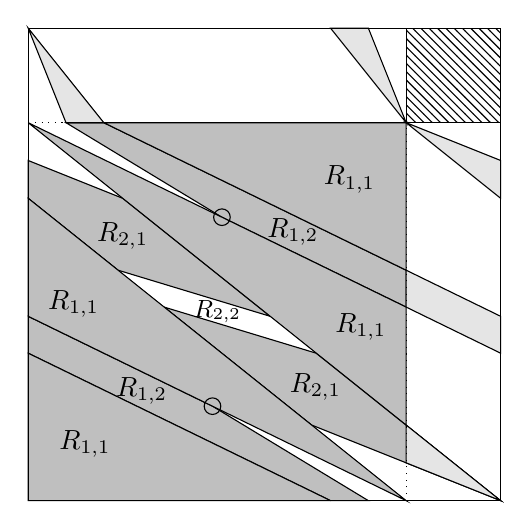
\begin{tikzpicture}[yscale=6,xscale=6]
	\def\p{0.8}
	\def\r{4}
	\def\s{5}
	\draw[pattern=north west lines, pattern color=black] (\p,\p) rectangle (1,1);
	\draw[fill=gray!50!white](1,0) -- (\p+\p-1,\p-\p^2) -- ({(\p^3-\p^2+\p+\p-1)/(1+\p^2)},{(\p^3-\p^2+\p)/(1+\p^2)}) -- ({1/(1+\p^2)},{(\p^3)/(1+\p^2)}) -- cycle;
	\draw[fill=gray!20!white](1,0) -- (\p,\p-\p^2) -- (\p,{(\p-\p^2)/2}) -- cycle;
	\draw[fill=gray!20!white](\p,\p) -- (1,\p^2) -- (1,{(\p+\p^2)/2}) -- cycle;
	\draw[fill=gray!50!white](0,\p^2) -- (0,{(\p+\p^2)/2}) -- (1-\p,\p^2) -- ({1-(\p)/(1+\p^2)},{(\p^2)/(1+\p^2)}) -- ({(\p^3+\p-1)/(1+\p^2)},{(\p)/(1+\p^2)}) -- cycle;
	\draw[fill=gray!50!white]({(\p-\p^2)/2},\p)--({(-\p^3 + \p^2 -\p - \p + 1)/(\p)+1},\p+\p-1)--(\p,{(\p-\p^2+\p^3)/(1+\p^2)})--(\p,{\p/(1+\p^2)})--({(\p-\p^2)},\p)--cycle;
	\draw[fill=gray!50!white](0,{\p^2/(1+\p^2)})--(0,{\p^3/(1+\p^2)})-- (\p^2,0) -- ({(\p^2+\p)/2},0)--({(\p^3 + \p -1)/(\p)},1-\p)--cycle;
	\draw[fill=gray!20!white](\p,\p)--(\p^2,1)--({(\p^2+\p)/2},1)--cycle;
	\draw[fill=gray!20!white](0,1)--({(\p-\p^2)},\p)--({(\p-\p^2)/2},\p)--cycle;
	\draw[fill=gray!20!white](\p,{\p/(1+\p^2)}) -- (1,{\p^2/(1+\p^2)}) -- (1,{\p^3/(1+\p^2)}) -- (\p,{(\p-\p^2+\p^3)/(1+\p^2)})--cycle;
	\draw [fill=gray!50!white] (\p-\p^2,\p)--(\p,{\p/(1+\p^2)})--(\p,\p)-- 
(\p-\p^2,\p);
	\draw [fill=gray!50!white] (0,\p)--(\p,{(\p-\p^2+\p^3)/(1+\p^2)})--(\p,{\p*(1-\p)}) -- (0,\p);
	\draw [fill=gray!50!white] (0,{\p^2/(1+\p^2)})--(0,\p^2)--(\p,0)--(0,{(\p^2/(1+\p^2)});
	\draw [fill=gray!50!white] (\p^2,0)--(0,0)--(0,{\p^3/(1+\p^2)})--(\p^2,0);
	\draw[dotted] (\p,0) --(\p,1);
	\draw[dotted] (0,\p) --(1,\p);
	\node at ({0.15*\p},{0.15*\p}) {$R_{1,1}$};
	\node at ({0.85*\p},{0.85*\p}) {$R_{1,1}$};
	\node at ({0.88*\p},{0.46*\p}) {$R_{1,1}$};
	\node at ({0.12*\p},{0.52*\p}) {$R_{1,1}$};
	\node at (0.76*\p,0.3*\p) {$R_{2,1}$};
	\node at (0.25*\p,0.7*\p) {$R_{2,1}$};
	\node at (0.3*\p,0.29*\p) {$R_{1,2}$};
	\node at (0.7*\p,0.71*\p) {$R_{1,2}$};
	\node at (0.5*\p,0.5*\p) {\small{$R_{2,2}$}};
	\draw ({(\p*\p*\p+\p-1)/\p},1-\p) {circle (0.5pt)};	
	\draw ({(-\p*\p*\p+\p*\p-\p+1)/\p},{2*\p-1}) {circle (0.5pt)};	
	\draw (0,0)--(1,0)--(1,1)--(0,1)--(0,0);
	\end{tikzpicture}

\end{document}